本章通过证明辛拓扑中的两个基本定理，说明伪全纯曲线工具的用法。这两个定理都可以把伪全纯曲线紧化模空间的直接分析同少量辛拓扑数据结合起来证明。第一个是格罗莫夫著名的非挤压定理。在它的证明中，某一类伪全纯曲线的存在性定理是最关键的分析要素。此外，证明还用到闭 $J$-全纯有理曲线之辛面积的正性与同调不变性。我们紧随格罗莫夫的原始证明方案。事后看来，这个存在性结果是
$S^2\times T^{2(n-1)}$ 上一点（闭）格罗莫夫--威腾不变量非平凡性的直接推论；该不变量由计数零维 $J$-全纯曲线模空间中的元素个数来定义。关于精细研究模空间本身并将其应用于环境辛 $4$-流形结构定理的更多非平凡例子，参见 (Gr85)、(Mc90)。

第二个定理是任意驯服辛流形上 $\Ham(M,\omega)$ 的霍费尔范数非退化性的证明。这个证明使用带拉格朗日边界条件、由含时哈密顿向量场扰动的柯西--黎曼方程之解模空间，并利用任意辛流形中“足够小”的紧拉格朗日子流形的自动可位移性。我们紧随吴龙根在 (Oh97c) 中对切卡诺夫证明 (Che98) 的简化。关于精细研究这个紧化模空间并将其卓越地应用于 $T^*S^{4k+1}$ 中 exotic 拉格朗日球的构造，参见穆罕默德·阿布扎伊德（Mohammed Abouzaid）的文章 (Ab12)。他的用法多少让人想起西蒙·柯万·唐纳森（Simon Kirwan Donaldson）最初利用反自对偶杨--米尔斯方程的模空间来完成其著名的 exotic $\mathbb R^4$ 构造 (Do86)。

一般而言，对这套工具更间接的应用会伴随某种同调代数。最突出的例子涉及由一族彼此相关的模空间构造出的弗洛尔同调型不变量。这需要 $J$-全纯曲线方程的各种变体：方程通常由哈密顿向量场或截面 $\mathcal H_{(j,J)}^{(0,1)}$ 的其他（非线性）零阶扰动所扰动，并且还允许映射的定义域成为穿孔黎曼曲面。弗洛尔同调理论是最著名的例子，其中这个扰动柯西--黎曼方程在同调代数的整套结构中得到系统使用。在我们对 $\Ham(M,\omega)$ 上霍费尔范数非退化性的证明里，则不涉及同调代数，而是展示如何直接使用由依赖于定义域的一族哈密顿向量场所扰动的柯西--黎曼方程之模空间。

\section{格罗莫夫非挤压定理}
\label{sec:gromov-non-squeezing-theorem}

本节紧随格罗莫夫的原始证明 (Gr85)，完整证明格罗莫夫著名的非挤压定理。

\begin{theorem}[非挤压定理]\label{thm:gromov-non-squeezing}
\stfhIndexRangeStart{I145}{ge^luo^mo^fu^fei^ji^ya^ding^li}{格罗莫夫非挤压定理（Gromov’s non-squeezing theorem）}
令 $\omega_0$ 为 $\mathbb C^n\cong\mathbb R^{2n}$ 上的标准辛形式，令 $B^{2n}(R)$ 为 $\mathbb C^n$ 中半径为 $R$ 的标准闭球。对 $D^2(r)\subset\mathbb C$，令
$Z^{2n}(r):=D^2(r)\times\mathbb C^{n-1}$。则对所有 $\epsilon>0$，存在辛嵌入
\[
 \Phi:(B^{2n}(R),\omega_0)\longrightarrow(Z^{2n}(r+\epsilon),\omega_0)
\]
当且仅当 $R<r$。
\end{theorem}

注意，如果 $R<r$，则对任何 $\epsilon>0$，总有 $B^{2n}(R)$ 到 $Z^{2n}(r+\epsilon)$ 的标准等距嵌入，故“如果”部分显然。因而只需证明“仅当”部分。我们将用反证法证明它。

\subsection{证明提纲}
\label{subsec:non-squeezing-proof-outline}

设 $R>r$，并任取 $\epsilon>0$ 使 $r+\epsilon<R$。反设存在辛嵌入
$\phi:B^{2n}(R)\to Z^{2n}(r+\epsilon/2)$。由于假设 $R>r+\epsilon$ 且
\begin{equation}
 \phi(B^{2n}(R))\subset\operatorname{Int}(Z^{2n}(r+\epsilon)),
 \label{eq:ch11-image-inside-cylinder}
\end{equation}
存在某个 $\delta>0$，使 $\phi$ 延拓为一个仍记作 $\phi$ 的辛嵌入
\[
 \phi:B^{2n}(R+\delta)\longrightarrow Z^{2n}(r+\epsilon).
\]

用 $\phi$ 把 $J_0$ 从 $B^{2n}(R+\delta)$ 推前到像
$\phi(B^{2n}(R+\delta))\subset Z^{2n}(r+\epsilon/2)$，并考虑 $\mathbb C^n$ 上满足
\[
 J_1=
 \begin{cases}
  \phi_*(J_0),&\text{在 }\phi(B^{2n}(R+\delta/2))\text{ 上},\\
  J_0,&\text{在 }\mathbb C^n\setminus
  \bigl(D^2(r+\epsilon)\times[-K+1,K-1]^{2(n-1)}\bigr)\text{ 上}
 \end{cases}
\]
的殆复结构 $J_1$；再把 $J_1$ 光滑延拓到剩余区域，使之仍与 $\omega$ 相容。

\begin{exercise}\label{ex:ch11-smooth-extension-almost-complex}
证明上述光滑延拓是可能的。（提示：使用极分解，并注意这个分解是典范的。）
\end{exercise}

上面的常数 $K>0$ 取成满足
\begin{equation}
 \phi(B^{2n}(R+\delta))
 \subset D^2(r+\epsilon/2)\times[-K+1,K-1]^{2(n-1)}.
 \label{eq:ch11-image-inside-compact-cylinder}
\end{equation}
下面是证明非挤压定理的三个关键步骤。

\medskip
\noindent\textbf{步骤 I（存在性定理）。}
证明存在 $J_1$-全纯映射
\[
 f:(D^2,\partial D^2)\longrightarrow
 \bigl(\mathbb C^n,\mathbb C^n\setminus\phi(B^{2n}(R+\delta))\bigr),
\]
使得
\begin{equation}
 \int_C\omega_0\leq\pi(r+\epsilon)^2,
 \label{eq:ch11-existence-area-bound}
\end{equation}
其中 $C=\operatorname{Image}f$，并且
\begin{equation}
 \phi(0)\in C.
 \label{eq:ch11-curve-through-center-image}
\end{equation}
这里回忆，$\pi(r+\epsilon)^2$ 是 $Z^{2n}(r+\epsilon)$ 中平坦圆盘的面积。

\medskip
\noindent\textbf{步骤 II（单调性公式）。}
\stfhIndex{I206}{dan^diao^xing^gong^shi}{单调性公式（monotonicity formula）}
现在考虑 $C$ 的原像，即
\[
 \phi^{-1}(C)\cap B^{2n}(R).
\]
因为
$\operatorname{Image}(f|_{\partial D^2})\subset
\mathbb C^n\setminus\phi(B^{2n}(R+\delta))$，
$\phi^{-1}(C)\cap B^{2n}(R)$ 定义了 $B^{2n}(R)$ 中一张\emph{通过原点}的\emph{真}曲面。此外，由于
$J_1|_{\phi(B^{2n}(R+\delta))}\equiv\phi_*J_0$ 且 $C$ 是 $J_1$-全纯曲线，
$\phi^{-1}(C)$ 是 $\mathbb C^n$ 上的 $J_0$-全纯曲线（从而关于 $\mathbb C^n$ 上的标准度量是\emph{极小曲面}）。经典单调性公式立即给出
\[
 \operatorname{Area}\bigl(\phi^{-1}(C)\cap B^{2n}(R)\bigr)\geq\pi R^2,
\]
因为 $\phi^{-1}\cap B^{2n}(R)$ 是一张通过原点的真 $J_0$-全纯（从而极小）曲面。参见图~\ref{fig:ch11-monotonicity}。

\begin{figure}[htbp]
 \centering
 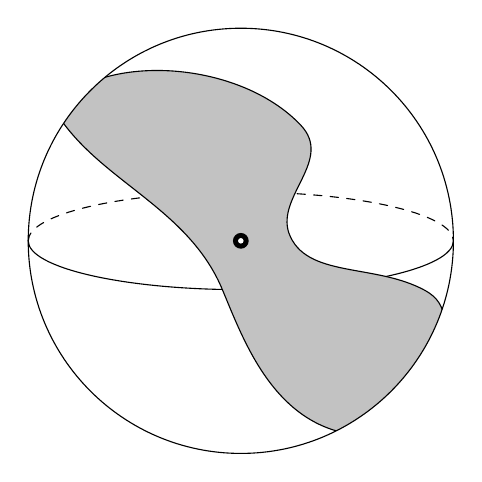
\begin{tikzpicture}[x=1cm,y=1cm,line cap=round,line join=round]
  \def\R{2.7}
  \draw[dashed] (-\R,0) arc[start angle=180,end angle=0,x radius=\R,y radius=.62];
  \draw (-\R,0) arc[start angle=180,end angle=360,x radius=\R,y radius=.62];
  \begin{scope}
    \clip (0,0) circle (\R);
    \path[fill=gray!48,draw=black]
      (-2.20,1.86)
      .. controls (-1.45,2.38) and (.05,2.22) .. (.76,1.47)
      .. controls (1.18,1.03) and (.45,.57) .. (.61,.10)
      .. controls (.82,-.48) and (1.70,-.28) .. (2.34,-.63)
      .. controls (2.98,-.98) and (2.23,-1.95) .. (1.37,-2.45)
      .. controls (.40,-2.28) and (.03,-1.25) .. (-.23,-.63)
      .. controls (-.64,.37) and (-1.68,.72) .. (-2.25,1.49)
      .. controls (-2.38,1.66) and (-2.33,1.78) .. cycle;
  \end{scope}
  \draw (0,0) circle (\R);
  \fill (0,0) circle (.10);
  \fill[white] (0,0) circle (.035);
\end{tikzpicture}

 \caption{单调性。}
 \label{fig:ch11-monotonicity}
\end{figure}

\medskip
\noindent\textbf{步骤 III（使用 $\omega_0$ 的 $J$-正性）。}
导出矛盾：依次使用式~\eqref{eq:ch11-existence-area-bound}、式~\eqref{eq:ch11-curve-through-center-image}、$\phi$ 是辛映射这一事实、变量替换、$\omega$ 在 $C$ 上的正性以及式~\eqref{eq:ch11-existence-area-bound}，得到
\[
 \begin{aligned}
 \pi R^2
 &\leq \operatorname{Area}\bigl(\phi^{-1}(C)\cap B^{2n}(R)\bigr)
  =\int_{\phi^{-1}(C)\cap B^{2n}(R)}\omega_0
  =\int_{\phi^{-1}(C)\cap B^{2n}(R)}\phi^*\omega_0\\
 &=\int_{C\cap\phi(B^{2n}(R))}\omega_0
  \leq\int_C\omega_0\leq\pi r^2.
 \end{aligned}
\]
这与假设 $R>r$ 矛盾，从而完成证明。

\subsection{存在性方案与一点 GW 不变量}
\label{subsec:existence-scheme-one-point-gw}

现在只剩证明步骤 I 中的存在性陈述。首先把 $J$-全纯圆盘的存在性陈述转化成\emph{闭}辛流形上一个更易处理的 $J$-全纯球面存在性问题。至此，我们在
$Z^{2n}(r)=D^2(r)\times\mathbb C^{n-1}$ 上有殆复结构 $J_1$，它在
\[
 \mathbb C^n\setminus
 \bigl(D^2(r+\epsilon)\times[-K+1,K-1]^{2(n-1)}\bigr)
 =:D_{r,\epsilon,K}
\]
上是标准的。因此，由 $J_0$ 的平移不变性，可以把 $D_{r,\epsilon,K}$ 上的 $J_1$ 推前到
\[
 D^2(r+\epsilon)\times T^{2(n-1)}(K),
\]
仍记为 $J_1$；这里 $T^{2(n-1)}(K)$ 是在 $[-K,K]$ 中把 $-K$ 与 $K$ 识别而得到的环面，即
\[
 T^{2(n-1)}(K)
 =\underbrace{S_K^1\times\cdots\times S_K^1}_{2(n-1)\text{ 个}},
 \qquad S_K^1=\mathbb R/K\mathbb Z.
\]
注意，由于 $\phi(B^{2n}(R+\delta))\subset D_{r,\epsilon,K}$，可把
$\phi(B^{2n}(R+\delta))$ 看作
\[
 D^2(r+\epsilon/2)\times T^{2(n-1)}(K)
\]
的子集。这个空间上相应的殆复结构 $J_1$ 在\emph{空间}边界附近仍是标准的。

现在用一个保面积映射把 $D^2(r+\epsilon/2)$ 嵌入
$S^2((r+\epsilon)/2)$，继而用辛映射
\[
 \psi\times\operatorname{id}:
 D^2(r+\epsilon/2)\times T^{2(n-1)}(K)
 \longrightarrow P_{r+\epsilon,K}
\]
把 $D^2(r+\epsilon/2)\times T^{2(n-1)}(K)$ 嵌入
\[
 P_{r+\epsilon,K}:=S^2\left(\frac{r+\epsilon}{2}\right)
 \times T^{2(n-1)}(K).
\]
以 $\omega_{r+\epsilon,K}=\omega_1\oplus\omega_2$ 表示 $P_{r+\epsilon,K}$ 上的乘积辛结构，其中 $\omega_1$ 和 $\omega_2$ 分别是
$S^2((r+\epsilon)/2)$ 与 $T^{2(n-1)}(K)$ 上的标准辛结构。现在把
$(\psi\times\operatorname{id})_*J_1$ 从
\[
 (\psi\times\operatorname{id})
 \bigl(D^2(r+\epsilon)\times T^{2(n-1)}(K)\bigr)
\]
延拓到整个
$P_{r+\epsilon,K}=S^2((r+\epsilon)/2)\times T^{2(n-1)}(K)$，使这个记为 $\widetilde J_1$ 的延拓与 $\omega_{r+\epsilon,K}$ 相容。注意
$\pi_2(P_{r+\epsilon,K})\cong\mathbb Z$，且同伦类
\[
 \left[S^2\left(\frac{r+\epsilon}{2}\right)\times\{\mathrm{pt}\}\right]
\]
生成 $\pi_2$。以 $A$ 表示这个同伦类，并令
$p_0\in P_{r+\epsilon,K}$ 为 $Z^{2n}(r+\epsilon)$ 中 $\phi(0)$ 所对应的点。

\medskip
\noindent\textbf{断言。}
为完成步骤 I，只需找到一张 $\widetilde J_1$-全纯球面 $\widetilde C$，使
\[
 [\widetilde C]=A\in\pi_2(P_{r+\epsilon,K}),
 \qquad p_0\in\widetilde C.
\]

\begin{proof}[断言的证明]
假设存在一张 $\widetilde J_1$-全纯球面 $\widetilde C$，并令
$u:S^2\to P_{r+\epsilon,K}$ 为表示 $\widetilde C$ 的映射，即
$\widetilde C=\operatorname{Image}(u)$。由于 $[\widetilde C]=A$，有
\[
 \int_{\widetilde C}\omega_{r+\epsilon,K}=\pi(r+\epsilon)^2.
\]
由
$[\widetilde C]=A=[S^2((r+\epsilon)/2)\times\{\mathrm{pt}\}]$，容易证明复合
\[
 \pi\circ u:S^2\longrightarrow S^2\left(\frac{r+\epsilon}{2}\right)
\]
是满射。现在，步骤 I 所需的曲线 $C$ 可以取作
\[
 C=(\psi\times\operatorname{id})^{-1}(\widetilde C)
 \subset D^2(r+\epsilon/2)\times T^{2(n-1)}(K),
\]
并可把它看作 $Z^{2n}(r+\epsilon/2)$ 的子集。显然，$C$ 是
$Z^{2n}(r+\epsilon/2)$ 中的真曲面；又因为本节开头假设
$\phi(B^{2n}(R+\delta))\subset Z^{2n}(r+\epsilon/2)$，所以
$C\cap\phi(B^{2n}(R+\delta))$ 在 $\phi(B^{2n}(R+\delta))$ 中定义一张真曲面。

此外，由于 $\psi\times\operatorname{id}$ 是辛映射，并由 $\widetilde J_1$ 的定义，
\[
 \begin{aligned}
 \int_C\omega_0
 &=\int_C(\psi\times\operatorname{id})^*\omega_{r+\epsilon,K}\\
 &=\int_{(\psi\times\operatorname{id})^{-1}(\widetilde C)}
     (\psi\times\operatorname{id})^*\omega_{r+\epsilon,K}\\
 &=\int_{\widetilde C\cap(\psi\times\operatorname{id})
   (D^2(r+\epsilon)\times T^{2(n-1)}(K))}\omega_{r+\epsilon,K}\\
 &\leq\int_{\widetilde C}\omega_{r+\epsilon,K}
 =\pi(r+\epsilon)^2,
 \end{aligned}
\]
这就证明了式~\eqref{eq:ch11-existence-area-bound}。这里，不等式来自
$p_0\in\widetilde C$、单调性公式和正性。
\end{proof}

于是，非挤压定理的证明已经约化为下面这个 $J_1$-全纯球面的一般存在性定理。

\begin{theorem}\label{thm:ch11-sphere-through-point}
令
$P_{r+\epsilon,K}=S^2((r+\epsilon)/2)\times T^{2(n-1)}(K)$，其辛形式为
$\omega_{r+\epsilon,K}=\omega_1\oplus\omega_2$；令 $J_\beta$ 为任意给定的相容殆复结构，并令 $p_0=(x_0,q_0)\in P_{r+\epsilon,K}$ 为任意给定点。令
\[
 A=\left[S^2\left(\frac{r+\epsilon}{2}\right)\times\{\mathrm{pt}\}\right]
\]
为 $\pi_2(P_{r+\epsilon,K})$ 的生成元。则存在 $J_\beta$-全纯球面
$u:S^2\to P_{r+\epsilon,K}$，使 $[u]=A$ 且 $p_0\in\operatorname{Image}(u)$。
\end{theorem}

先给出下面这个一般定义。

\begin{definition}\label{def:ch11-j-simple-class}
\stfhIndex{I248}{dan^chun^lei}{单纯类（simple class）}
\stfhSubIndex{I249}{dan^chun^lei}{单纯类（simple class）}{a^dan^chun}{$A$-单纯（$A$-simple）}
\stfhSubIndex{I250}{dan^chun^lei}{单纯类（simple class）}{j^dan^chun}{$J$-单纯（$J$-simple）}
令 $J$ 为 $(M,\omega)$ 的相容殆复结构。如果不存在
\[
 A=\sum_{j=1}^N A_j,\qquad N\geq2,
\]
这样的分解，使每个 $A_j$ 都容许一条非平凡 $J$-全纯曲线，则称同伦类 $A$ 是\emph{$J$-单纯}的。如果这对每个 $J\in\mathcal J_\omega$ 都成立，则称同伦类 $A$ 是\emph{单纯}的。
\end{definition}

\begin{lemma}\label{lem:ch11-fiber-sphere-class-simple}
同伦类 $A=[S^2\times\{\mathrm{pt}\}]$ 是单纯的。
\end{lemma}

\begin{proof}
如果存在上述分解，则有
\[
 [\omega](A)=\sum_{j=1}^N[\omega](A_j).
\]
但是，如果 $A_j$ 容许某条非常值 $J$-全纯曲线，则
\[
 [\omega](A_j)>0,
 \qquad\text{从而}\qquad
 [\omega](A_j)\geq\pi(r+\epsilon)^2.
\]
另一方面，$[\omega](A)=\pi(r+\epsilon)^2$，所以这种分解不可能存在。
\end{proof}

$A$ 的单纯性立即给出下面的推论。

\begin{corollary}\label{cor:ch11-universal-moduli-injective}
集合
\[
 \widetilde{\mathcal M}(M;A)
 :=\{(u,J)\mid J\in\mathcal J_\omega,
 \overline\partial_Ju=0,\ [u]=A\}
\]
等于其开子集 $\widetilde{\mathcal M}^{\mathrm{inj}}(M;A)$。特别地，它是光滑无穷维（巴拿赫）流形，并且投影
\[
 \Pi_A:\widetilde{\mathcal M}(M;A)\longrightarrow\mathcal J_\omega
\]
是指标为 $2c_1(A)+2n=4+2n$ 的光滑弗雷德霍姆映射。
\end{corollary}

现在回到定理~\ref{thm:ch11-sphere-through-point} 的证明。为证明它，我们将使用 PDE 中著名连续性方法的一个版本。从
$S^2((r+\epsilon)/2)\times T^{2(n-1)}(K)$ 上的标准（可积）乘积结构 $J_\alpha$ 出发。

\begin{lemma}\label{lem:ch11-product-structure-a-regular}
$S^2((r+\epsilon)/2)\times T^{2(n-1)}(K)$ 上的乘积结构 $J_\alpha$ 是
$A$-正则的，其中
$A=[S^2((r+\epsilon)/2)\times\{\mathrm{pt}\}]$，并且
\[
 \widetilde{\mathcal M}(J_\alpha;A)
 =\left\{f:S^2\to P_{r+\epsilon,K}\mathrel{\Big|}
 \begin{array}{l}
 f(z)=(f_1(z),q),\quad q\in T^{2(n-1)}(K),\\
 f_1:S^2\to S^2((r+\epsilon)/2)\text{ 是双全纯映射}
 \end{array}\right\}.
\]
\end{lemma}

\begin{exercise}\label{ex:ch11-product-structure-regular}
证明这个引理。
\end{exercise}

注意，指标公式 $2(2+n)=2n+4$ 与上述引理中对
$\widetilde{\mathcal M}(J_\alpha;A)$ 的显式描述一致。回忆我们要找的是通过给定点 $p_0$ 的 $J_\beta$-全纯球面。因此考虑评价映射
\[
 \operatorname{ev}_A:\mathcal M_1(J_\alpha;A)\longrightarrow P,
 \qquad \operatorname{ev}_A(f,z)=f(z),
\]
其中
\[
 \mathcal M_1(J_\alpha;A)
 =\widetilde{\mathcal M}(J;A)\times S^2/PSL(2;\mathbb C)
\]
是类 $A$ 中单标记点稳定映射的模空间。$\mathcal M_1(J_\alpha;A)$ 的维数为
\[
 2(c_1(A)+n)+2-6=2c_1(A)+2n-4.
\]
在引理~\ref{lem:ch11-product-structure-a-regular} 的乘积结构 $J_\alpha$ 情形，$c_1(A)=2$，因而可直接看出这个维数等于 $2n$。事实上，可以证明下面的引理。

\begin{lemma}\label{lem:ch11-product-evaluation-diffeomorphism}
对乘积结构 $J_\alpha$，$\mathcal M_1(J_\alpha;A)$ 是紧 $2n$-流形，并且评价映射
\[
 \operatorname{ev}_A:\mathcal M_1(J_\alpha;A)\longrightarrow P_{r+\epsilon,K}
\]
是微分同胚。特别地，它具有非零 $\mathbb Z_2$-度数。
\end{lemma}

\begin{exercise}\label{ex:ch11-product-evaluation-diffeomorphism}
证明这个引理。
\end{exercise}

现在考虑定理~\ref{thm:ch11-sphere-through-point} 中给定的 $J_\beta$。一般而言，$J_\beta$ 未必 $A$-正则，所以选择一列 $A$-正则的 $J_i$，使
\[
 J_i\longrightarrow J_\beta\qquad(i\to\infty)
\]
在 $C^\infty$ 拓扑中成立。对每个固定的 $i$，考虑一条道路
$\overline J=\{J_t\}_{0\leq t\leq1}$，满足 $J_0=J_\alpha$、$J_1=J_i$，以及交换图
\[
\begin{tikzpicture}[baseline=(current bounding box.center),>=Stealth]
 \node (top) at (0,1.4) {$\mathcal M_1(M;A)$};
 \node (left) at (-2.4,0) {$[0,1]$};
 \node (right) at (2.4,0) {$\mathcal J_\omega$};
 \draw[->] (top) -- node[right] {$\Pi_A$} (right);
 \draw[->] (left) -- node[above] {$\overline J$} (right);
\end{tikzpicture}
\]
其中
\[
 \mathcal M_1(M;A)=\bigcup_{J\in\mathcal J_\omega}
 \{J\}\times\mathcal M_1(J;A).
\]
由相对横截性定理，可以选择与 $\Pi_A$ 横截并满足
$\overline J_0=J_\alpha$、$\overline J_1=J_i$ 的道路 $\overline J$。于是族
\[
 \Pi_A^{-1}(\overline J)
 =\bigcup_{t\in[0,1]}\{t\}\times\mathcal M_1(J_t;A)
\]
定义了 $\mathcal M_1(J_0;A)$ 与 $\mathcal M_1(J_1;A)$ 之间的光滑配边。

此外，评价映射
\[
 \operatorname{ev}_A^0\amalg\operatorname{ev}_A^1:
 \mathcal M_1(J_0;A)\amalg\mathcal M_1(J_1;A)
 \longrightarrow P_{r+\epsilon,K}
\]
延拓为参数化评价映射
\[
 \begin{gathered}
 \operatorname{Ev}_A:
 \mathcal M_1(\overline J;A)\times_GS^2
 \longrightarrow P_{r+\epsilon,K}\times[0,1],\\
 \mathcal M_1(\overline J;A)
 :=\bigcup_{t\in[0,1]}\{t\}\times\mathcal M_1(J_t;A),
 \end{gathered}
\]
其定义为
\[
 \operatorname{Ev}_A(t;f_t,J_t,z)=(f_t(z),t),
\]
并且它也是光滑的。

在上述情形中，如果能证明 $\mathcal M_1(\overline J;A)$ 紧，它就给出
$\mathcal M_1(J_\alpha;A)$ 与 $\mathcal M_1(J_i;A)$ 之间的\emph{紧}配边，故评价映射
\[
 \operatorname{ev}_A^0:\mathcal M_1(J_\alpha;A)
 \longrightarrow P_{r+\epsilon,K}\times\{0\}
\]
和
\[
 \operatorname{ev}_A^1:\mathcal M_1(J_i;A)
 \longrightarrow P_{r+\epsilon,K}\times\{1\}
\]
必有相同的 $\mathbb Z_2$-度数。因此，由引理 5.6，
$\operatorname{ev}_A^0$ 的 $\mathbb Z_2$-度数为 $1$，所以
\[
 \operatorname{ev}_A^1:\mathcal M_1(J_i;A)\longrightarrow P_{r+\epsilon,K}
\]
具有非零 $\mathbb Z_2$-度数，特别地，它是满射。这又蕴含存在一条通过
$p_0$ 的 $J_i$-全纯曲线，记为 $u_i$。现在，如果能证明导数 $du_i$ 的一致估计
\begin{equation}
 \max_{z\in S^2}|du_i(z)|\leq C,
 \label{eq:ch11-uniform-derivative-bound}
\end{equation}
对所有 $i$ 都成立，那么重参数化后可以取极限，得到满足
$p_0\in\operatorname{Image}u_\beta$ 的 $J_\beta$-全纯球面 $u_\infty$；这将完成定理~\ref{thm:ch11-sphere-through-point}，从而完成非挤压定理的证明。

上述两个紧性陈述都将是格罗莫夫紧性定理的推论；下一小节会描述这个定理。把格罗莫夫紧性定理用于当前情形时，要用到一致面积界
\eqref{eq:ch11-uniform-derivative-bound}，以及同伦类
$A=[S^2((r+\epsilon)/2)\times\{\mathrm{pt}\}]$ 是\emph{单纯}的这一事实。

\subsection{光滑收敛的证明}
\label{subsec:proof-smooth-convergence}

本小节的主要目标是证明上一小节留下的两个紧性陈述。先考虑下面的命题。

\begin{proposition}\label{prop:ch11-parameterized-moduli-compact}
令
$P=S^2((r+\epsilon)/2)\times T^{2(n-1)}(K)$，并令
$A\in\pi_2(P)$ 如前。则对任意道路
$\overline J=\{J_t\}_{0\leq t\leq1}\subset\mathcal J_\omega$，
$\mathcal M_1(\overline J;A)$ 都是紧的。此外，如果固定两个 $A$-正则的结构
$J_0=J_\alpha$、$J_1=J_\gamma$，则存在一条光滑道路 $\overline J$，使
$\mathcal M_1(\overline J;A)$ 成为紧光滑流形。
\end{proposition}

这是格罗莫夫紧性定理的参数化版本。

\begin{theorem}[格罗莫夫收敛定理]\label{thm:ch11-gromov-convergence}
设 $J_\gamma\to J_\infty$ 是 $\mathcal J_\omega$ 中的收敛序列。对任意具有一致面积界
\[
 \operatorname{Area}(f_\gamma)<C
\]
的 $J_\gamma$-全纯映射序列 $f_\gamma:S^2\to P$，存在一个子列，使非参数化曲线
$C_\gamma=\operatorname{Image}f_\gamma$ 弱收敛到尖点曲线
$C_\infty=\{C_{\infty,\ell}\}_{1\leq\ell\leq N}$，并满足
\begin{enumerate}[label=(\arabic*)]
 \item $\displaystyle
 \operatorname{Area}(C_\infty)
 =\lim_{\gamma\to\infty}\operatorname{Area}(C_\infty)
 =\sum_{\ell=1}^N\operatorname{Area}(C_{\infty,\ell})$；
 \item $\displaystyle
 [C_\infty]=\sum_{\ell=1}^N[C_{\infty,\ell}]\quad\text{在 }\pi_2(P)\text{ 中}$；
 \item $C_\infty$ 是连通尖点曲线。
\end{enumerate}
此外，如果 $N=1$，即 $C_\infty$ 是一条真正的光滑曲线，那么必要时作重参数化后，子列 $f_\gamma$ 在 $C^\infty$ 意义下收敛到极限 $f_\infty$。
\end{theorem}

\begin{exercise}\label{ex:ch11-gromov-convergence-from-stable-maps}
这是亏格零稳定映射集合 $\mathcal M_1(M,J;\leq C)$ 的紧性定理之直接推论。验证这一断言。
\end{exercise}

现在可以证明命题~\ref{prop:ch11-parameterized-moduli-compact}。

\begin{proof}[命题~\ref{prop:ch11-parameterized-moduli-compact} 的证明]
因为 $\mathcal M_1(\overline J;A)$ 是
$\mathcal M(\overline J;A)=\widetilde{\mathcal M}(\overline J;A)/G$ 上的 $S^2$-丛，只需证明 $\mathcal M(\overline J;A)$ 紧。令
$(f_i,J_{t_i})$ 为 $\mathcal M(\overline J;A)$ 中的序列。我们有一致面积界
$\omega(f_i)\leq C(A)$。于是上述紧性定理蕴含：$f_i$ 有一个仍记为 $f_i$ 的子列，使非参数化曲线 $C_i=\operatorname{Image}f_i$ 收敛到尖点曲线
\[
 C_\infty=\sum_{\ell=1}^N C_{\infty,\ell}.
\]
再取子列，可以假设 $t_i\to t_\infty$。然而，由于 $A$ 单纯，根据上一小节末尾的论证，$N$ 不可能大于 $1$；所以重参数化后，子列 $f_i$ 收敛到一条 $J_{t_\infty}$-全纯曲线。这证明了 $\mathcal M(\overline J;A)$ 紧。若选择与命题 5.2 中的投影
\[
 \Pi_2:\mathcal M(M;A)\longrightarrow\mathcal J_\omega
\]
横截的道路 $\overline J$，则由横截性定理得到最后一个陈述。
\end{proof}

给定一列 $A$-正则的 $J_i$，使 $J_i\to J_\beta$，其中 $J_\beta$ 如定理~\ref{thm:ch11-sphere-through-point}。
对每个 $J_i$ 使用命题 6.1 和存在性方案，得到一列通过 $p_0$ 的 $J_i$-全纯球面 $f_i$。再次利用面积界和 $A$ 的单纯性，上述格罗莫夫紧性定理保证极限 $f_\infty$（在重参数化后）存在，并且 $f_\infty$ 是 $J_\beta$-全纯的且
$p_0\in\operatorname{Image}f_\infty$。这最终完成了非挤压定理的证明。
\stfhIndexRangeEnd{I145}{ge^luo^mo^fu^fei^ji^ya^ding^li}{格罗莫夫非挤压定理（Gromov’s non-squeezing theorem）}
